% Copyright 2004 by Till Tantau <tantau@users.sourceforge.net>.
%
% In principle, this file can be redistributed and/or modified under
% the terms of the GNU Public License, version 2.
%
% However, this file is supposed to be a template to be modified
% for your own needs. For this reason, if you use this file as a
% template and not specifically distribute it as part of a another
% package/program, I grant the extra permission to freely copy and
% modify this file as you see fit and even to delete this copyright
% notice. 

\documentclass{beamer}

% There are many different themes available for Beamer. A comprehensive
% list with examples is given here:
% http://deic.uab.es/~iblanes/beamer_gallery/index_by_theme.html

\usetheme{CambridgeUS}


%%%%%%%%%%%%%%%%%%%%%%%%%%%%%%%%%%%%%
\usepackage{algorithm}
\usepackage{algorithmic}

\newcommand{\cvar}{\text{CVaR}}
\newcommand{\var}{\text{VaR}}

\newcommand{\envelope}{\mathcal{U}_{\cvar}(\alpha, P(\cdot | x, a))}

\newcommand{\indicator}{\mathbb{1}}
\renewcommand{\exp}{\mathbb{E}}
\newcommand{\expval}[1]{\mathbb{E}\left[ {#1} \right]}

\newcommand{\given}[1][]{\:#1\vert\:}

\newcommand{\bround}[1]{\left( {#1} \right)}
\newcommand{\bsquare}[1]{\left[ {#1} \right]}
\newcommand{\braces}[1]{\left\{ {#1} \right\}}

\newcommand{\interpI}{\mathcal{I}}
\newcommand{\dt}{\text{d}}
%%%%%%%%%%%%%%%%%%%%%%%%%%%%%%%%%%%%



\title{Risk-averse Distributional Reinforcement Learning}

% A subtitle is optional and this may be deleted
\subtitle{A CVaR optimization approach}

\author{Silvestr Stanko\inst{1}}
% - Give the names in the same order as the appear in the paper.
% - Use the \inst{?} command only if the authors have different
%   affiliation.

\institute[] % (optional, but mostly needed)
{
  \inst{1}%
  Department of Computer Science\\
  Czech Technical University
%  \and
%  \inst{2}%
%  Department of Theoretical Philosophy\\
%  University of Elsewhere
  }
% - Use the \inst command only if there are several affiliations.
% - Keep it simple, no one is interested in your street address.

\date{\today}
% - Either use conference name or its abbreviation.
% - Not really informative to the audience, more for people (including
%   yourself) who are reading the slides online

\subject{Theoretical Computer Science}
% This is only inserted into the PDF information catalog. Can be left
% out. 

% If you have a file called "university-logo-filename.xxx", where xxx
% is a graphic format that can be processed by latex or pdflatex,
% resp., then you can add a logo as follows:

% \pgfdeclareimage[height=0.5cm]{university-logo}{university-logo-filename}
% \logo{\pgfuseimage{university-logo}}

% Delete this, if you do not want the table of contents to pop up at
% the beginning of each subsection:
%\AtBeginSubsection[]
%{
%  \begin{frame}<beamer>{Outline}
%    \tableofcontents[currentsection,currentsubsection]
%  \end{frame}
%}

% Let's get started
\begin{document}

\begin{frame}
  \titlepage
\end{frame}

\begin{frame}{Outline}
  \tableofcontents
  % You might wish to add the option [pausesections]
\end{frame}

% Section and subsections will appear in the presentation overview
% and table of contents.
\section{Introduction}

\subsection{Motivation}

\begin{frame}{Motivation}
\begin{figure}
    \centering
    \begin{minipage}{0.45\textwidth}
        \centering
        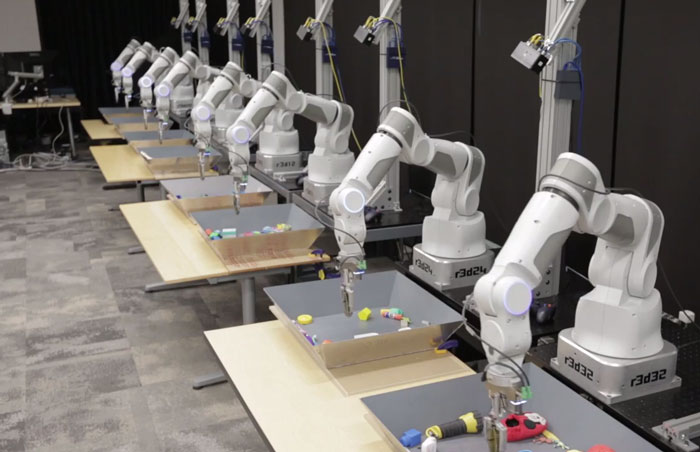
\includegraphics[width=0.87\linewidth]{../gfx/Deep-Learning-for-Robots.jpg}
        \caption{Robotics}
    \end{minipage}\hfill
    \begin{minipage}{0.45\textwidth}
        \centering
        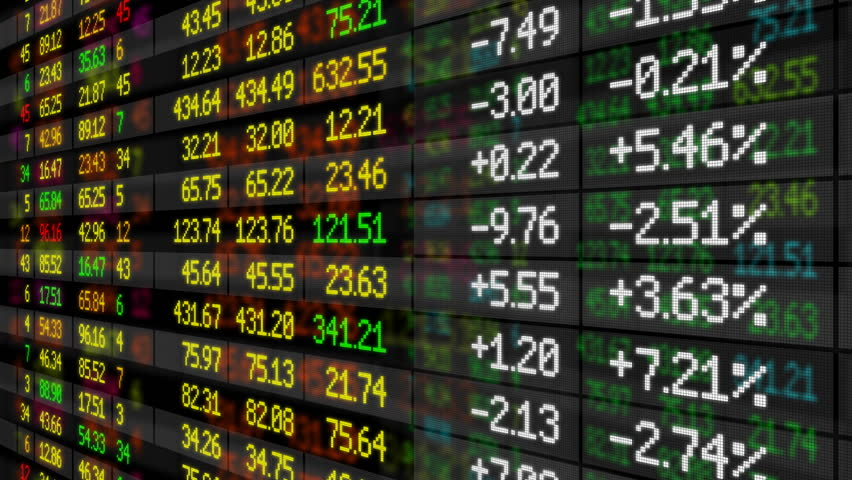
\includegraphics[width=\linewidth]{../gfx/stock_market.jpg}
        \caption{Finance}
    \end{minipage}
\end{figure}

\begin{figure}
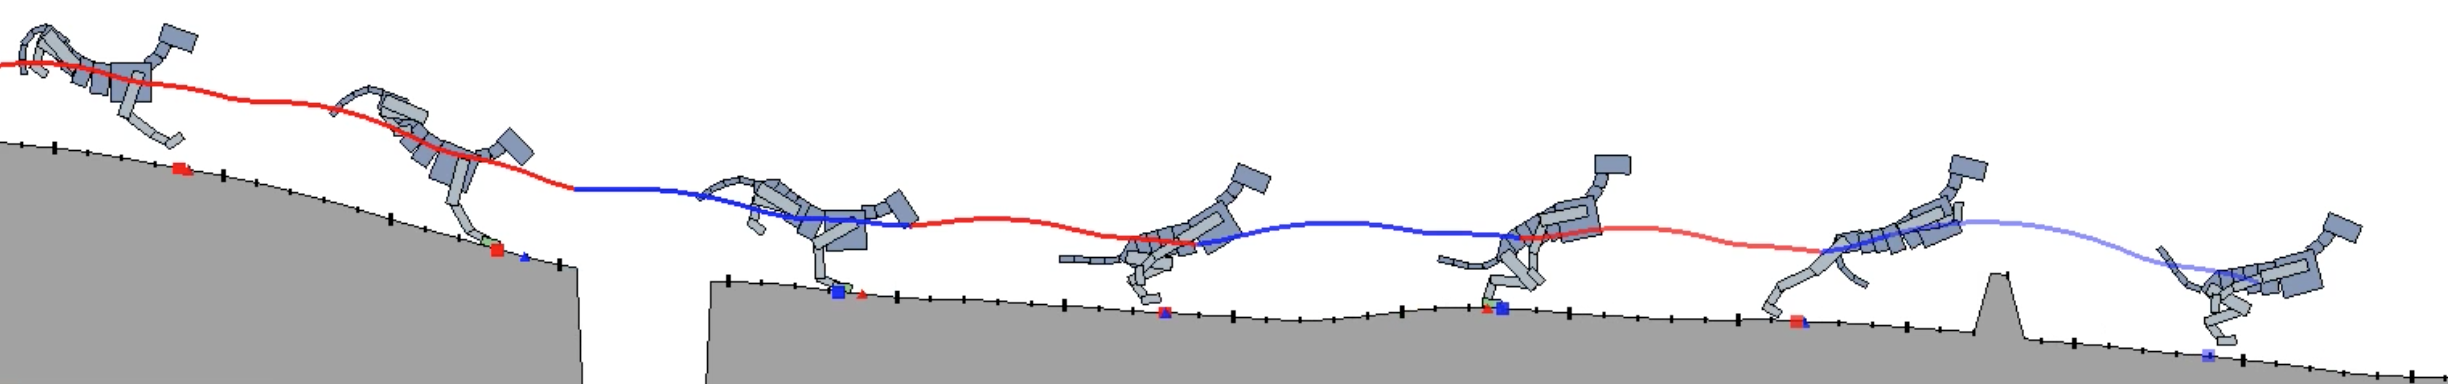
\includegraphics[width=\linewidth]{../gfx/running_tiger.png}
\caption{AI safety}
\end{figure}


\end{frame}

\subsection{Conditional Value-at-Risk}


\begin{frame}{Value-at-Risk}

\begin{itemize}
\item Easy to understand
\item Historically the most used risk-measure
\item Undesirable computational properties
\item Does not differentiate between large and catastrophic losses
\end{itemize}

$$
\text{VaR}_\alpha(Z)=F^{-1}(\alpha)=\max\left\lbrace z | F(z) \le \alpha \right\rbrace
$$

\end{frame}

\begin{frame}{Conditional Value-at-Risk}

\begin{itemize}
\item Coherent risk measure
\item Basel Committee on Banking Supervision $\to$ CVaR
\item Equivalent to robustness
\end{itemize}

$$
\text{CVaR}_\alpha(Z) = \dfrac{1}{\alpha}\int_0^\alpha F^{-1}_Z(\beta) \text{d}\beta = \dfrac{1}{\alpha}\int_0^\alpha \text{VaR}_\beta(Z) \text{d}\beta
$$

\end{frame}


\begin{frame}{VaR, CVaR}
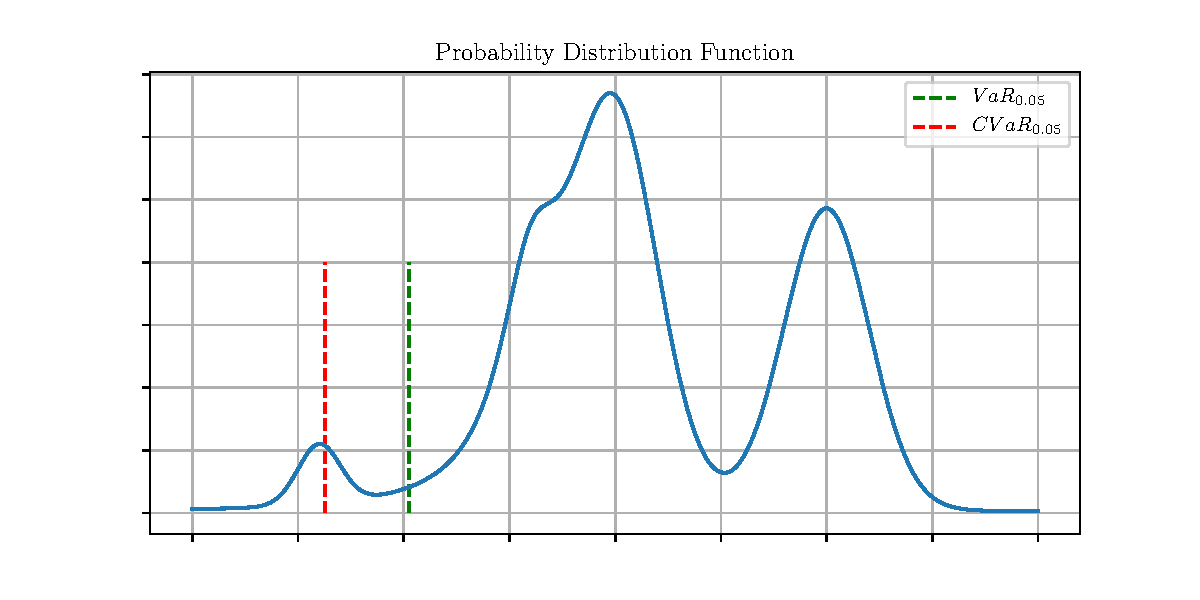
\includegraphics[width=\linewidth]{../gfx/pdf.pdf}
\end{frame}


\begin{frame}{Reinforcement Learning}

\begin{definition}
An MDP is a 5-tuple $\mathcal{M} = (\mathcal{X}, \mathcal{A}, R, P, \gamma)$, where $\mathcal{X}$ and $\mathcal{A}$ are the finite state and action spaces.

$R(x, a) \in [R_{\min}, R_{\max}]$ is a random variable representing the reward generated by being in state $x$ and selecting action $a$; $P(\cdot|x, a)$ is the transition probability distribution;
$\gamma \in [0, 1)$ is a discount factor. 

We also assume we are given a starting state $x_0$.
\end{definition}

\end{frame}


\begin{frame}{Goal}

\begin{definition}
$Z^\pi(x_t)$ Is a random variable representing the discounted reward along a trajectory generated by the MDP by following the policy $\pi$, starting at state $x_t$.
$$Z^\pi(x_{t})=\sum_{t=0}^\infty \gamma^tR(x_t,\pi(x_t))$$

\end{definition}

\begin{block}{Reinforcement Learning with CVaR}
For a given $\alpha$, our goal is to find a globally optimal policy $\pi^*$

$$\pi^* = \text{arg}\max_\pi CVaR^\pi_\alpha(Z^\pi(x_0))$$
\end{block}
\end{frame}

% You can reveal the parts of a slide one at a time
% with the \pause command:
%\begin{frame}{Second Slide Title}
%  \begin{itemize}
%  \item {
%    First item.
%    \pause % The slide will pause after showing the first item
%  }
%  \item {   
%    Second item.
%  }
%  % You can also specify when the content should appear
%  % by using <n->:
%  \item<3-> {
%    Third item.
%  }
%  \item<4-> {
%    Fourth item.
%  }
%  % or you can use the \uncover command to reveal general
%  % content (not just \items):
%  \item<5-> {
%    Fifth item. \uncover<6->{Extra text in the fifth item.}
%  }
%  \end{itemize}
%\end{frame}

\section{CVaR Value Iteration}
\subsection{Previous results}

\begin{frame}{Value Iteration}

\begin{theorem}[CVaR decomposition]
For any $t\geq 0$, denote by $Z  = (Z_{t+1},Z_{t+2},\dots)$ the reward sequence from time $t+1$ onwards. The conditional CVaR under policy $\pi$ obeys the following decomposition:
$$CVaR_\alpha\bround{Z^\pi(x, a)} = \min_{\xi \in \envelope} \sum_{x'} p(x'| x, a)\xi(x') CVaR_{\xi(x')\alpha}\bround{Z^\pi(x')}$$
\end{theorem}

\begin{theorem}[CVaR Value Iteration]
The following Bellman operator is a contraction:
$$\mathbf{T}V(x, y) = \max_a \bsquare{ R(x, a) + \gamma \min_{\xi} \sum_{x'} p(x'| x, a)\xi(x') V\bround{x', y\xi(x')}}$$
\end{theorem}

\end{frame}

\begin{frame}{CVaR Value Iteration}

\begin{theorem}[CVaR Value Iteration]
The following Bellman operator is a contraction:
$$\mathbf{T}V(x, y) = \max_a \bsquare{ R(x, a) + \gamma \min_{\xi} \sum_{x'} p(x'| x, a)\xi(x') V\bround{x', y\xi(x')}}$$
\end{theorem}

\vspace{1cm}

The operator $\mathbf{T}$ describes the following relationship:

$$\mathbf{T} CVaR_y(Z(x))=\max_a \bsquare{R(x, a) + \gamma CVaR_{y}(Z(x, a))}$$

\end{frame}


\begin{frame}{Linear interpolation}

Computing operator $\mathbf{T}$ s intractable, as the state-space is continuous. A solution would be to approximate the operator with linear interpolation.

\begin{theorem}
The function $\alpha\cvar_\alpha$ is convex. The operator $\mathbf{T}_\interpI$ is a contraction.

$$\interpI_{x}[V](y)=y_iV(x,y_{i})+\frac{y_{i+1}V(x,y_{i+1})-y_iV(x,y_{i})}{y_{i+1}-y_i}(y-y_i)$$

$$\mathbf{T}_\interpI V(x, y) = \max_a \bsquare{ R(x, a) + \gamma \min_{\xi} \sum_{x'} p(x'| x, a)\dfrac{\interpI_{x'} [V](y\xi(x'))}{y}}$$

\end{theorem}

This iteration can be formulated and solved as a linear program.

\end{frame}


\begin{frame}
\center
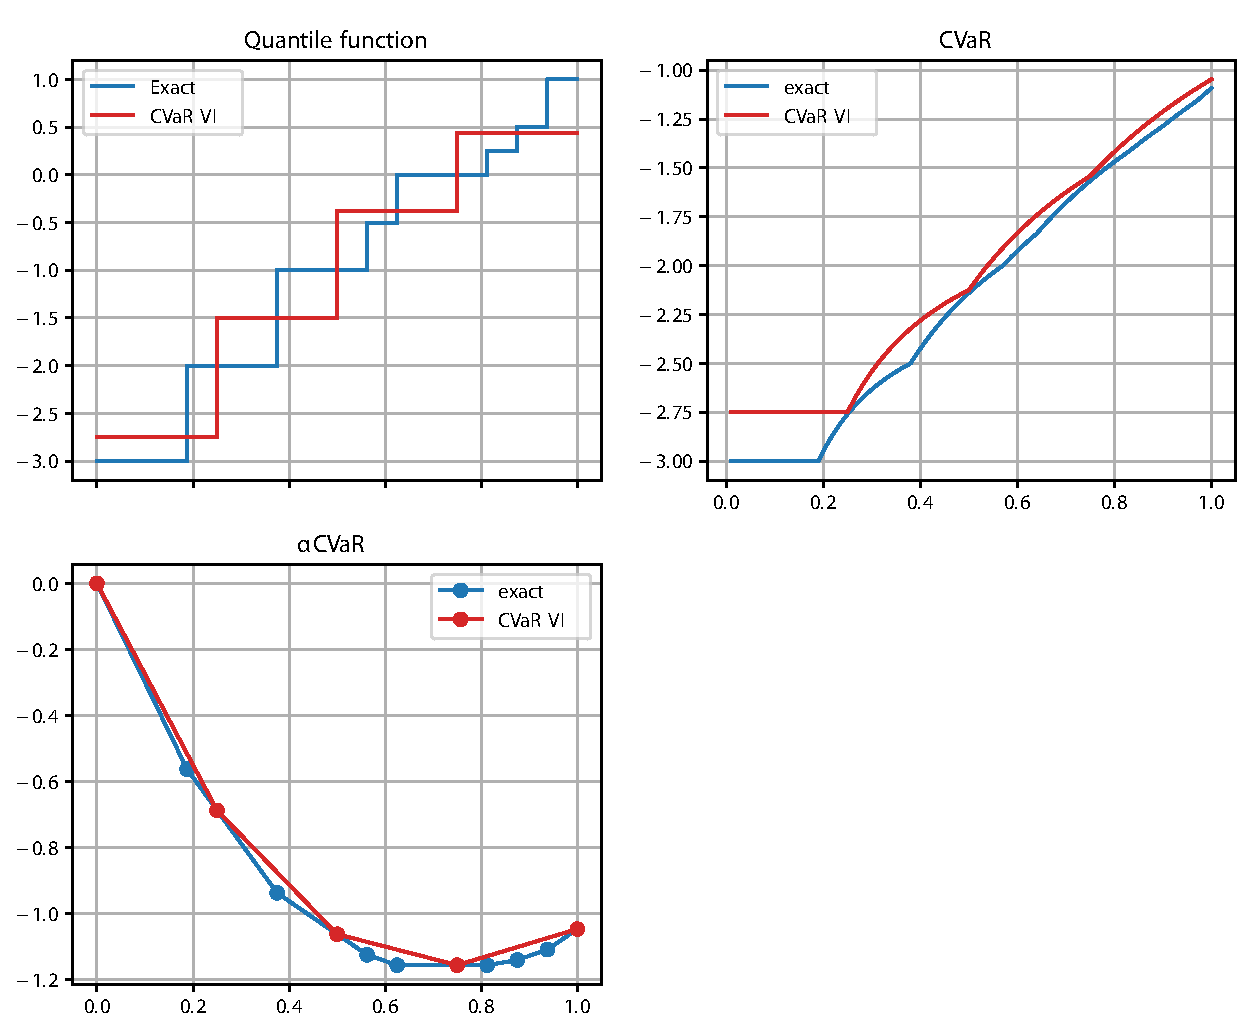
\includegraphics[width=0.8\linewidth]{../gfx/exactvarcvar.pdf}
\end{frame}



\subsection{Linear-time improvement}

\begin{frame}{$\alpha\cvar_\alpha$ duality}
\begin{lemma}
Any discrete distribution has a piecewise linear $\alpha\cvar_\alpha$ function. Similarly, any a piecewise linear $\alpha\cvar_\alpha$ function can be seen as representing a certain discrete distribution.
\end{lemma}

\begin{block}{$\alpha\cvar_\alpha 	\Leftarrow \var$}
$$\dfrac{\partial}{\partial \alpha} \alpha \cvar_\alpha(Z) = \dfrac{\partial}{\partial \alpha} \int_0^\alpha VaR_\beta(Z) d\beta = VaR_\alpha(Z)$$
\end{block}


\begin{block}{$\alpha\cvar_\alpha 	\Rightarrow \var$}
$$\alpha \cvar_\alpha(Z) = \int_0^\alpha VaR_\beta(Z) \dt \beta$$
\end{block}

\end{frame}


\begin{frame}{Linear-time Computation}

\begin{theorem}
Solution to minimization problem present in the CVaR Value Iteration can be computed by setting
$$\xi ( x' ) = \dfrac{F_{x'}(F^{-1}_x(\alpha))}{\alpha} $$

The computational complexity is $O(n\cdot m)$ where $n$ is the number of transition states and $m$ is the number of atoms.
\end{theorem}
\end{frame}

\begin{frame}{Next state CVaR computation}
\center
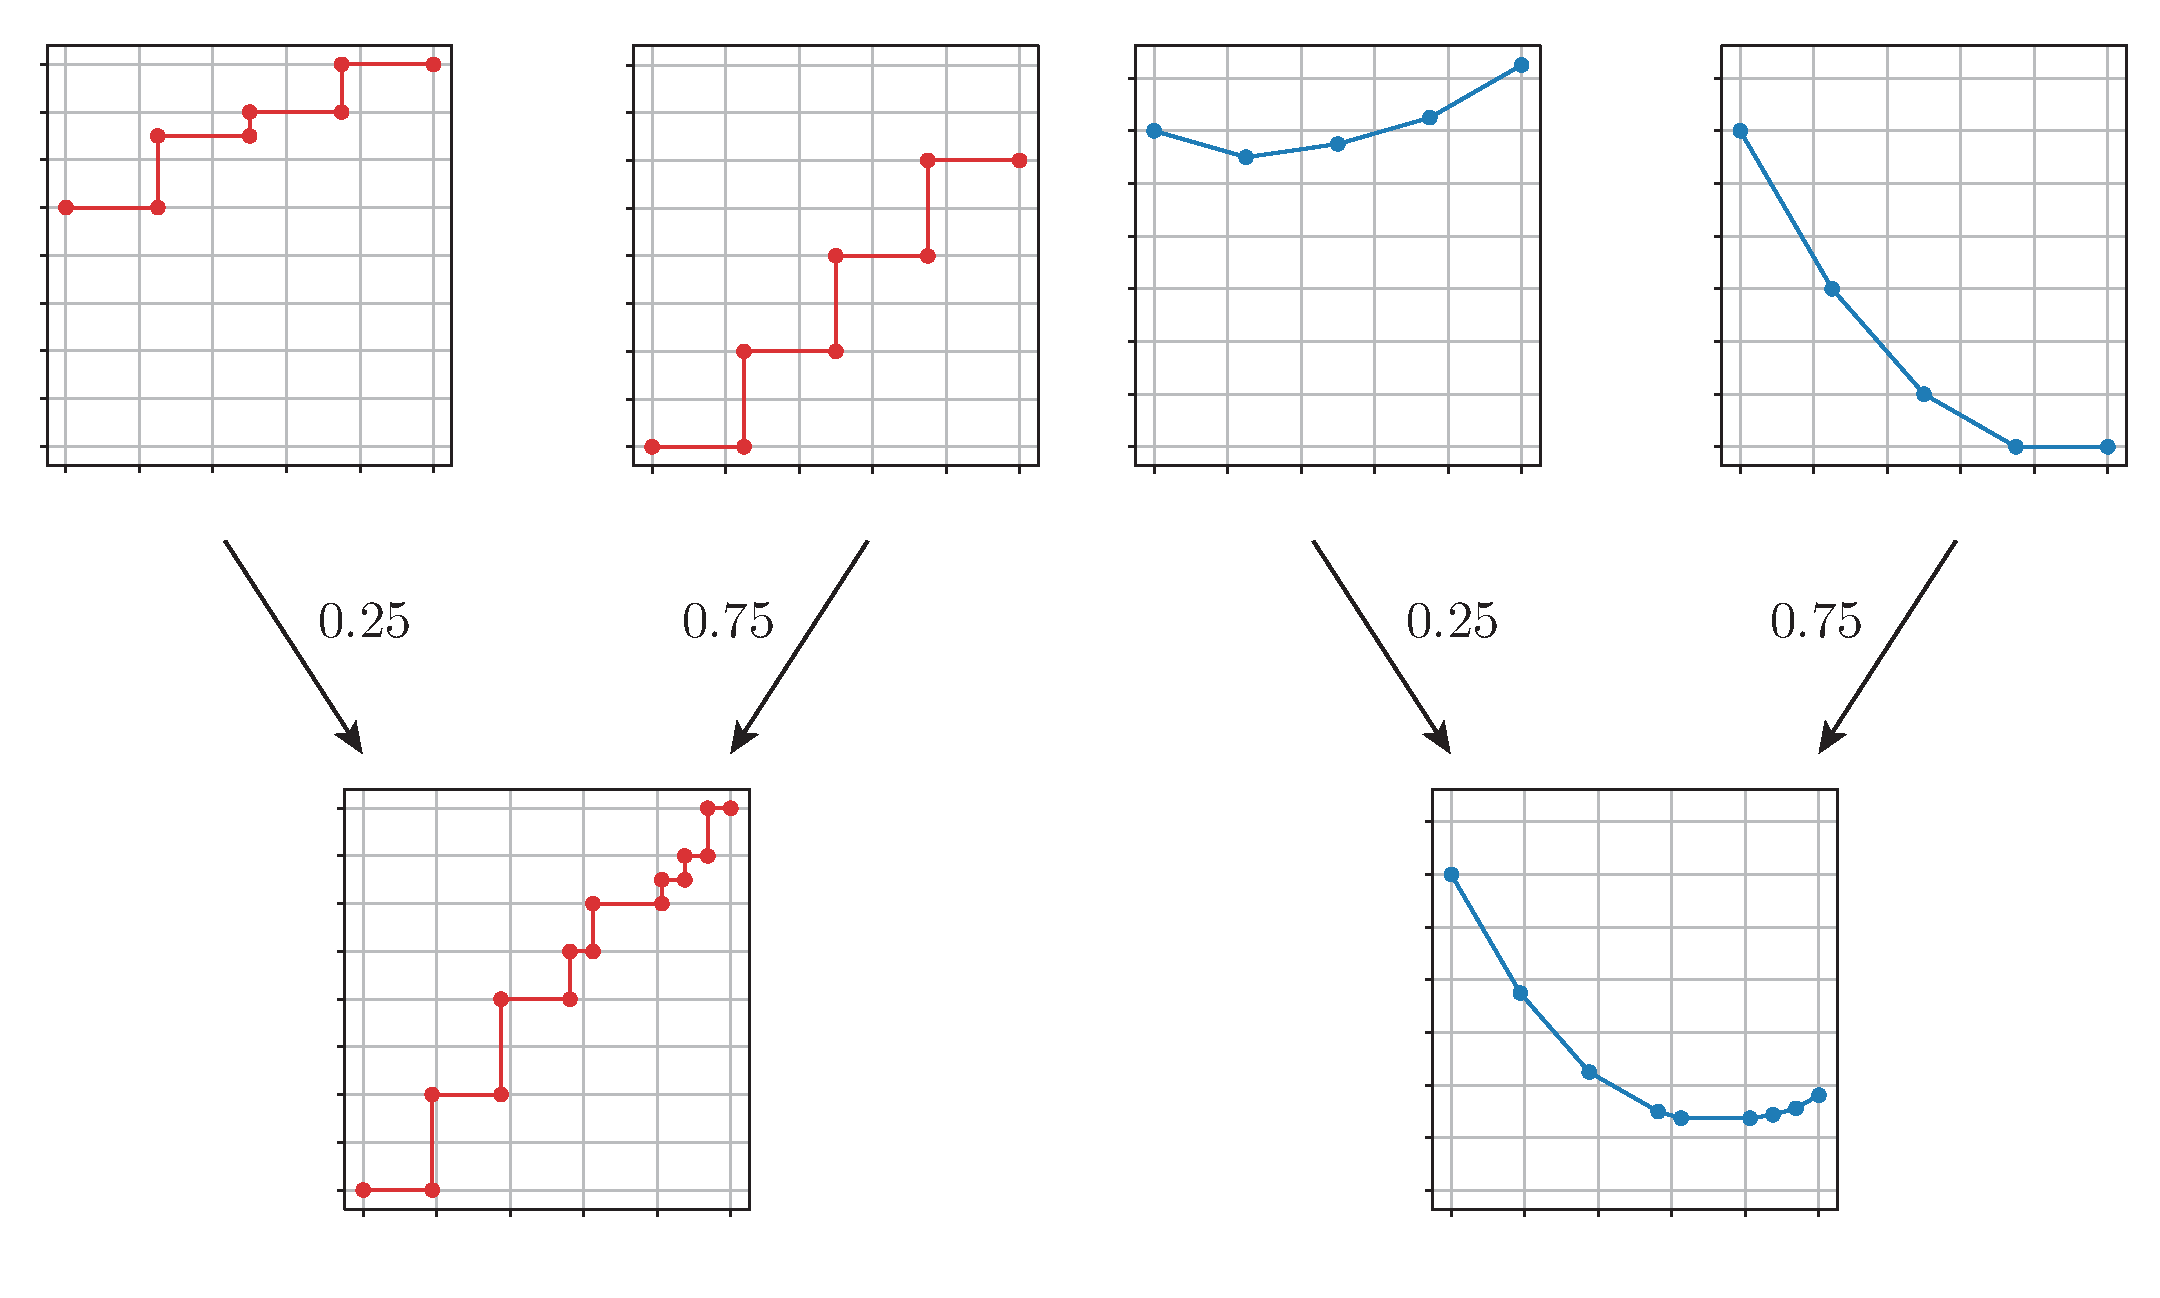
\includegraphics[width=\linewidth]{../gfx/multivarvar.pdf}
\end{frame}

\section{Other Results}

\begin{frame}{VaR-based Policy Improvement}
\begin{theorem}
Let $\pi$ be a fixed policy, $\alpha \in (0, 1]$. By following policy $\pi'$ from the following algorithm, we will improve $CVaR_\alpha(Z)$ in expectation:

$$CVaR_\alpha(Z^\pi) \le CVaR_\alpha(Z^{\pi'})$$
\end{theorem}


\begin{algorithmic}
    \STATE \textbf{input} $\alpha, x_0, \gamma$
    \STATE $a = \text{arg}\max_a CVaR_\alpha(Z(x_0, a))$
    \STATE $s = VaR_\alpha(Z(x_0, a))$
    \STATE $x_t, r_t = \text{envTransition}(x_0, a)$
    \WHILE{$x_t$ is not terminal}
    	\STATE $s = \dfrac{s-r_t}{\gamma}$
    	\STATE $a = \text{arg}\max_a \mathbb{E}\left[(Z(x_t, a)-s)^- \right]$
    	\STATE $x_t, r_t = \text{envTransition}(x_t, a)$
   	\ENDWHILE
\end{algorithmic}

\end{frame}


\begin{frame}{Implementations}
\center
\url{https://github.com/Silvicek/policy-improvement}

\vspace{1cm}

\url{https://github.com/Silvicek/distributional-dqn}

\end{frame}

\begin{frame}{TODO}

\begin{itemize}
\item CVaR Q-learning
\begin{itemize}
\item (?) Use Wasserstein distance with quantile improvement
\item (?) Extend the VaR-based algorithm
\item (?) Combine with quantile regression
\end{itemize}

\item Experiments
\begin{itemize}
\item Value Iteration + Q-learning
\item Deep Q-learning
\end{itemize}



\end{itemize}



\end{frame}

%\begin{frame}{Blocks}
%\begin{block}{Block Title}
%You can also highlight sections of your presentation in a block, with it's own title
%\end{block}
%\begin{theorem}
%There are separate environments for theorems, examples, definitions and proofs.
%\end{theorem}
%\begin{example}
%Here is an example of an example block.
%\end{example}
%\end{frame}



% Placing a * after \section means it will not show in the
% outline or table of contents.
%\section*{Summary}
%
%\begin{frame}{Summary}
%  \begin{itemize}
%  \item
%    The \alert{first main message} of your talk in one or two lines.
%  \item
%    The \alert{second main message} of your talk in one or two lines.
%  \item
%    Perhaps a \alert{third message}, but not more than that.
%  \end{itemize}
%  
%  \begin{itemize}
%  \item
%    Outlook
%    \begin{itemize}
%    \item
%      Something you haven't solved.
%    \item
%      Something else you haven't solved.
%    \end{itemize}
%  \end{itemize}
%\end{frame}



% All of the following is optional and typically not needed. 
%\appendix
%\section<presentation>*{\appendixname}
%\subsection<presentation>*{For Further Reading}

%\begin{frame}[allowframebreaks]
%  \frametitle<presentation>{For Further Reading}
%    
%  \begin{thebibliography}{10}
%    
%  \beamertemplatebookbibitems
%  % Start with overview books.
%
%  \bibitem{Author1990}
%    A.~Author.
%    \newblock {\em Handbook of Everything}.
%    \newblock Some Press, 1990.
% 
%    
%  \beamertemplatearticlebibitems
%  % Followed by interesting articles. Keep the list short. 
%
%  \bibitem{Someone2000}
%    S.~Someone.
%    \newblock On this and that.
%    \newblock {\em Journal of This and That}, 2(1):50--100,
%    2000.
%  \end{thebibliography}
%\end{frame}

\end{document}


